%%%
%
% $Autor: Adhiraj $
% $Datum: 2021-05-14 $
% $Pfad:  $
% $Dateiname: SBOM
% $Version: 4620 $
%
% !TeX spellcheck = de_DE/GB
% !TeX program = pdflatex
% !BIB program = biber/bibtex
% !TeX encoding = utf8
%
%%%




\chapter{Software Requirement and Bill Of Materials}
\section{Software Requirement and Bill Of Materials }

\begin{table}[H]
	
	\begin{tabular}{||m{1.6cm}|m{1.3cm}|m{3.5cm}|m{2.7cm}|m{2.1cm}|m{3cm}|m||}
		
		\hline
		
		\textbf{Software} & \textbf{Version} & \textbf{License}& \textbf{Dependencies}  & \textbf{Libraries}  \\
		
		\hline
		
		Arduino IDE & 2.1.2 &  Open-source (available under General Public License)& Java Runtime Environment (JRE) to run  &  ArduinoBLE and ArduinoLSM9DS1 \\
		
		
		\hline
		
		Python  & 3.11.3 & Open-source (Python Software Foundation License) & doesn't have strict dependencies & NumPy, Pandas and Matplotlib \\
		
		\hline
		
		Tensor Flow & 2.15.0 & Open-source (Apache License 2.0) & Hardware libraries  &  TensorFlow Lite Micro \\
		
		\hline
		
		Pycharm  & 2023.1.2 (Community Edition) & Open-source (Apache License 2.0) & Java Runtime Environment  & Python Interpreter and Git Integration \\
		
		\hline
		
	\end{tabular}
	
	\caption {Software Requirements}
	\label{Table 5.2}
\end{table}

Table \ref{Table 7.2}, titled Software Requirements, outlines the essential tools and environments required for the effective development and implementation of the project. All the listed software is compatible with Windows, macOS (Mac), and Linux operating systems.

\begin{enumerate}
	
	\item \textbf{Arduino IDE on PC}
	
	The Arduino IDE serves as the primary programming interface for the Arduino Nano 33 BLE Sense Board. This open-source, official Arduino software enables users to edit, upload, and compile code for Arduino modules. Built on the Java platform, the IDE supports various Arduino modules and is compatible with both C and C++ programming languages. The Arduino Nano 33 BLE Sense relies on the Arduino IDE, which is the most commonly used development environment for Arduino boards and can be utilized both online and offline \cite{Arduino:2015}. Different versions of the software are available for macOS, Linux, and Windows operating systems. Users can access these software packages through the following link: \url{https://www.arduino.cc/en/software}. Notably, during installation, it is crucial to ensure that the necessary drivers for the Arduino Nano 33 BLE Sense Board are also installed \cite{Fezari:2018}.
	
	
	\item \textbf{Python}
	
	The project's coding requirements are fulfilled using Python, a highly versatile programming language distributed under the Python Software Foundation License. To streamline dependency management, it is advisable to establish a virtual environment \cite{PyCharm:2021}.  
	
	Table \ref{Tab:PythonPackages} outlines the key Python packages utilized in the project, detailing their versions, licenses, and dependencies. The "Dependencies" column specifies the required dependencies for each package, including any version constraints. For a comprehensive list of the packages, refer to the \href{../Documents/MagicWand/ML23-06-Magic-Wand-with-an-Arduino-Nano-33-BLE-sense/Sourcecode/Requirements.txt}{\texttt{Requirements.txt}} file.
	
	\item \textbf{Tensorflow}
	
	TensorFlow, an open-source library developed by Google, is primarily designed for deep learning but also supports machine learning applications. It processes data in multi-dimensional arrays, making it highly efficient for managing large datasets. TensorFlow may have hardware dependencies, and utilizing GPU support requires specific configurations. The library provides APIs for Python and C++ and can also be integrated with R and Java. One of TensorFlow's key advantages is its compatibility with both GPUs and CPUs, enabling versatile performance optimization. Licensed under the Apache License 2.0, users should carefully review hardware compatibility and configuration requirements as detailed in TensorFlow's documentation \cite{Ramsundar:2018}.
	
	\begin{table}[H]
		\centering
		\begin{tabular}{||m{2cm}|m{1.5cm}|m{3.5cm}|m{3.5cm}|m||}
			\hline
			\textbf{Package} & \textbf{Version} & \textbf{License} & \textbf{Dependencies} \\
			\hline
			Python & 2.9 & Open Source (PSF) & - \\
			\hline
			tensorflow & 2.15.0 & Open Source (Apache 2.0) & numpy (>=1.16.6) \\
			& & & gast (=0.3.3) \\
			& & & keras-preprocessing (=1.1.0) \\
			& & & keras-applications (=1.0.8) \\
			& & & tensorboard (=2.6.0) \\
			& & & termcolor (>=1.1.0) \\
			& & & wrapt (>=1.11.1) \\
			& & & absl-py (>=0.7.0) \\
			& & & grpcio (>=1.8.6) \\
			& & & astunparse (=1.6.3) \\
			& & & google-pasta (=0.2.0) \\
			& & & h5py (>=2.9.0) \\
			& & & opt-einsum (=3.3.0) \\
			& & & protobuf (>=3.12.2) \\
			\hline
			numpy & 1.26.2 & Open Source (BSD) & - \\
			\hline
			Matplotlib & 3.8.2 & Open Source (PSF) & cycler (>=0.10.0) \\
			& & & kiwisolver (>=1.0.1) \\
			& & & numpy (>=1.15) \\
			& & & Pillow (>=6.2.0) \\
			& & & pyparsing (>=2.0.3) \\
			& & & six (>=1.5) \\
			\hline
			Pandas & 2.1.4 & Open Source (BSD) & numpy (>=1.16.6) \\
			& & & python-dateutil (>=2.7.3) \\
			& & & pytz (>=2015.7) \\
			\hline
			six & 1.16.0 & MIT & - \\
			\hline
		\end{tabular}
		\caption{Python packages and dependencies}
		\label{Tab:PythonPackages}
	\end{table}
	
	\begin{itemize}
		\item \textbf{Python 3.9:}
		\begin{itemize}
			\item Python is the programming language in which your project is written. Python 3.9 is a stable and widely used version with numerous improvements and features compared to Python 2. Using the latest version is recommended for compatibility, security, and access to the latest language features.
		\end{itemize}
		
		\item \textbf{TensorFlow 2.7.0:}
		\begin{itemize}
			\item TensorFlow is a popular open-source machine learning library. In your project, it's likely used for developing and training machine learning models for keyword spotting. TensorFlow provides tools for building neural networks and processing audio data, which are essential for speech-related tasks.
			\begin{itemize}
				\item Note that \texttt{TensorFlow Lite} is used to facilitate the deployment of machine learning models on edge devices with limited resources. The framework provides tools like the TensorFlow Lite Converter, which optimizes models for memory-constrained devices, and supports quantization to reduce model size and improve execution speed on CPUs \cite{Goldsborough:2016}.
			\end{itemize}
		\end{itemize}
		
		\item \textbf{NumPy 1.26.2:}
		\begin{itemize}
			\item NumPy is a fundamental library for scientific computing in Python. It provides support for large, multi-dimensional arrays and matrices, along with mathematical functions to operate on these arrays. In your project, NumPy may be used for efficient handling and manipulation of numerical data, which is common in machine learning tasks.
		\end{itemize}
		
		\item \textbf{Matplotlib 3.8.2:}
		\begin{itemize}
			\item Matplotlib is a plotting library for creating visualizations in Python. In the context of your project, it may be used for visualizing data, training progress, or results. For instance, you might use Matplotlib to create graphs or spectrograms of audio data.
		\end{itemize}
		
		\item \textbf{six 1.16.0:}
		\begin{itemize}
			\item The \texttt{six} library is used for writing code that is compatible with both Python 2 and Python 3. However, since you are using Python 3.9, the need for \texttt{six} might be limited. It's possible that it's used in parts of the codebase that were originally designed to be compatible with Python 2.
		\end{itemize}
		
		\item \textbf{Pandas 1.3.2:}
		\begin{itemize}
			\item Pandas is a powerful data manipulation and analysis library. It provides data structures like DataFrames that are useful for handling structured data. In your project, Pandas might be used for organizing and preprocessing data before training machine learning models.
		\end{itemize}
	\end{itemize}
	
	\item \textbf{Pycharm}
	
	PyCharm offers a robust development environment for Python programming. It requires a valid Java Runtime Environment (JRE) and can be installed by downloading it from the JetBrains website. The Community Edition is free, open-source, and distributed under the Apache License 2.0. Proper configuration of PyCharm to use the Python interpreter from the project's virtual environment is crucial for optimal functionality \cite{JetBrains:2023}.
	
\end{enumerate}

Collectively, these software components constitute a comprehensive and well-integrated toolset for the successful realization of the project.

\begin{table}[H]
	
	\begin{tabular}{||m{4cm}|m{6.0cm}|m{2cm}|m||}
		
		\hline
		
		\textbf{Hardware} & \textbf{Description} & \textbf{Quantity} \\
		
		\hline
		
		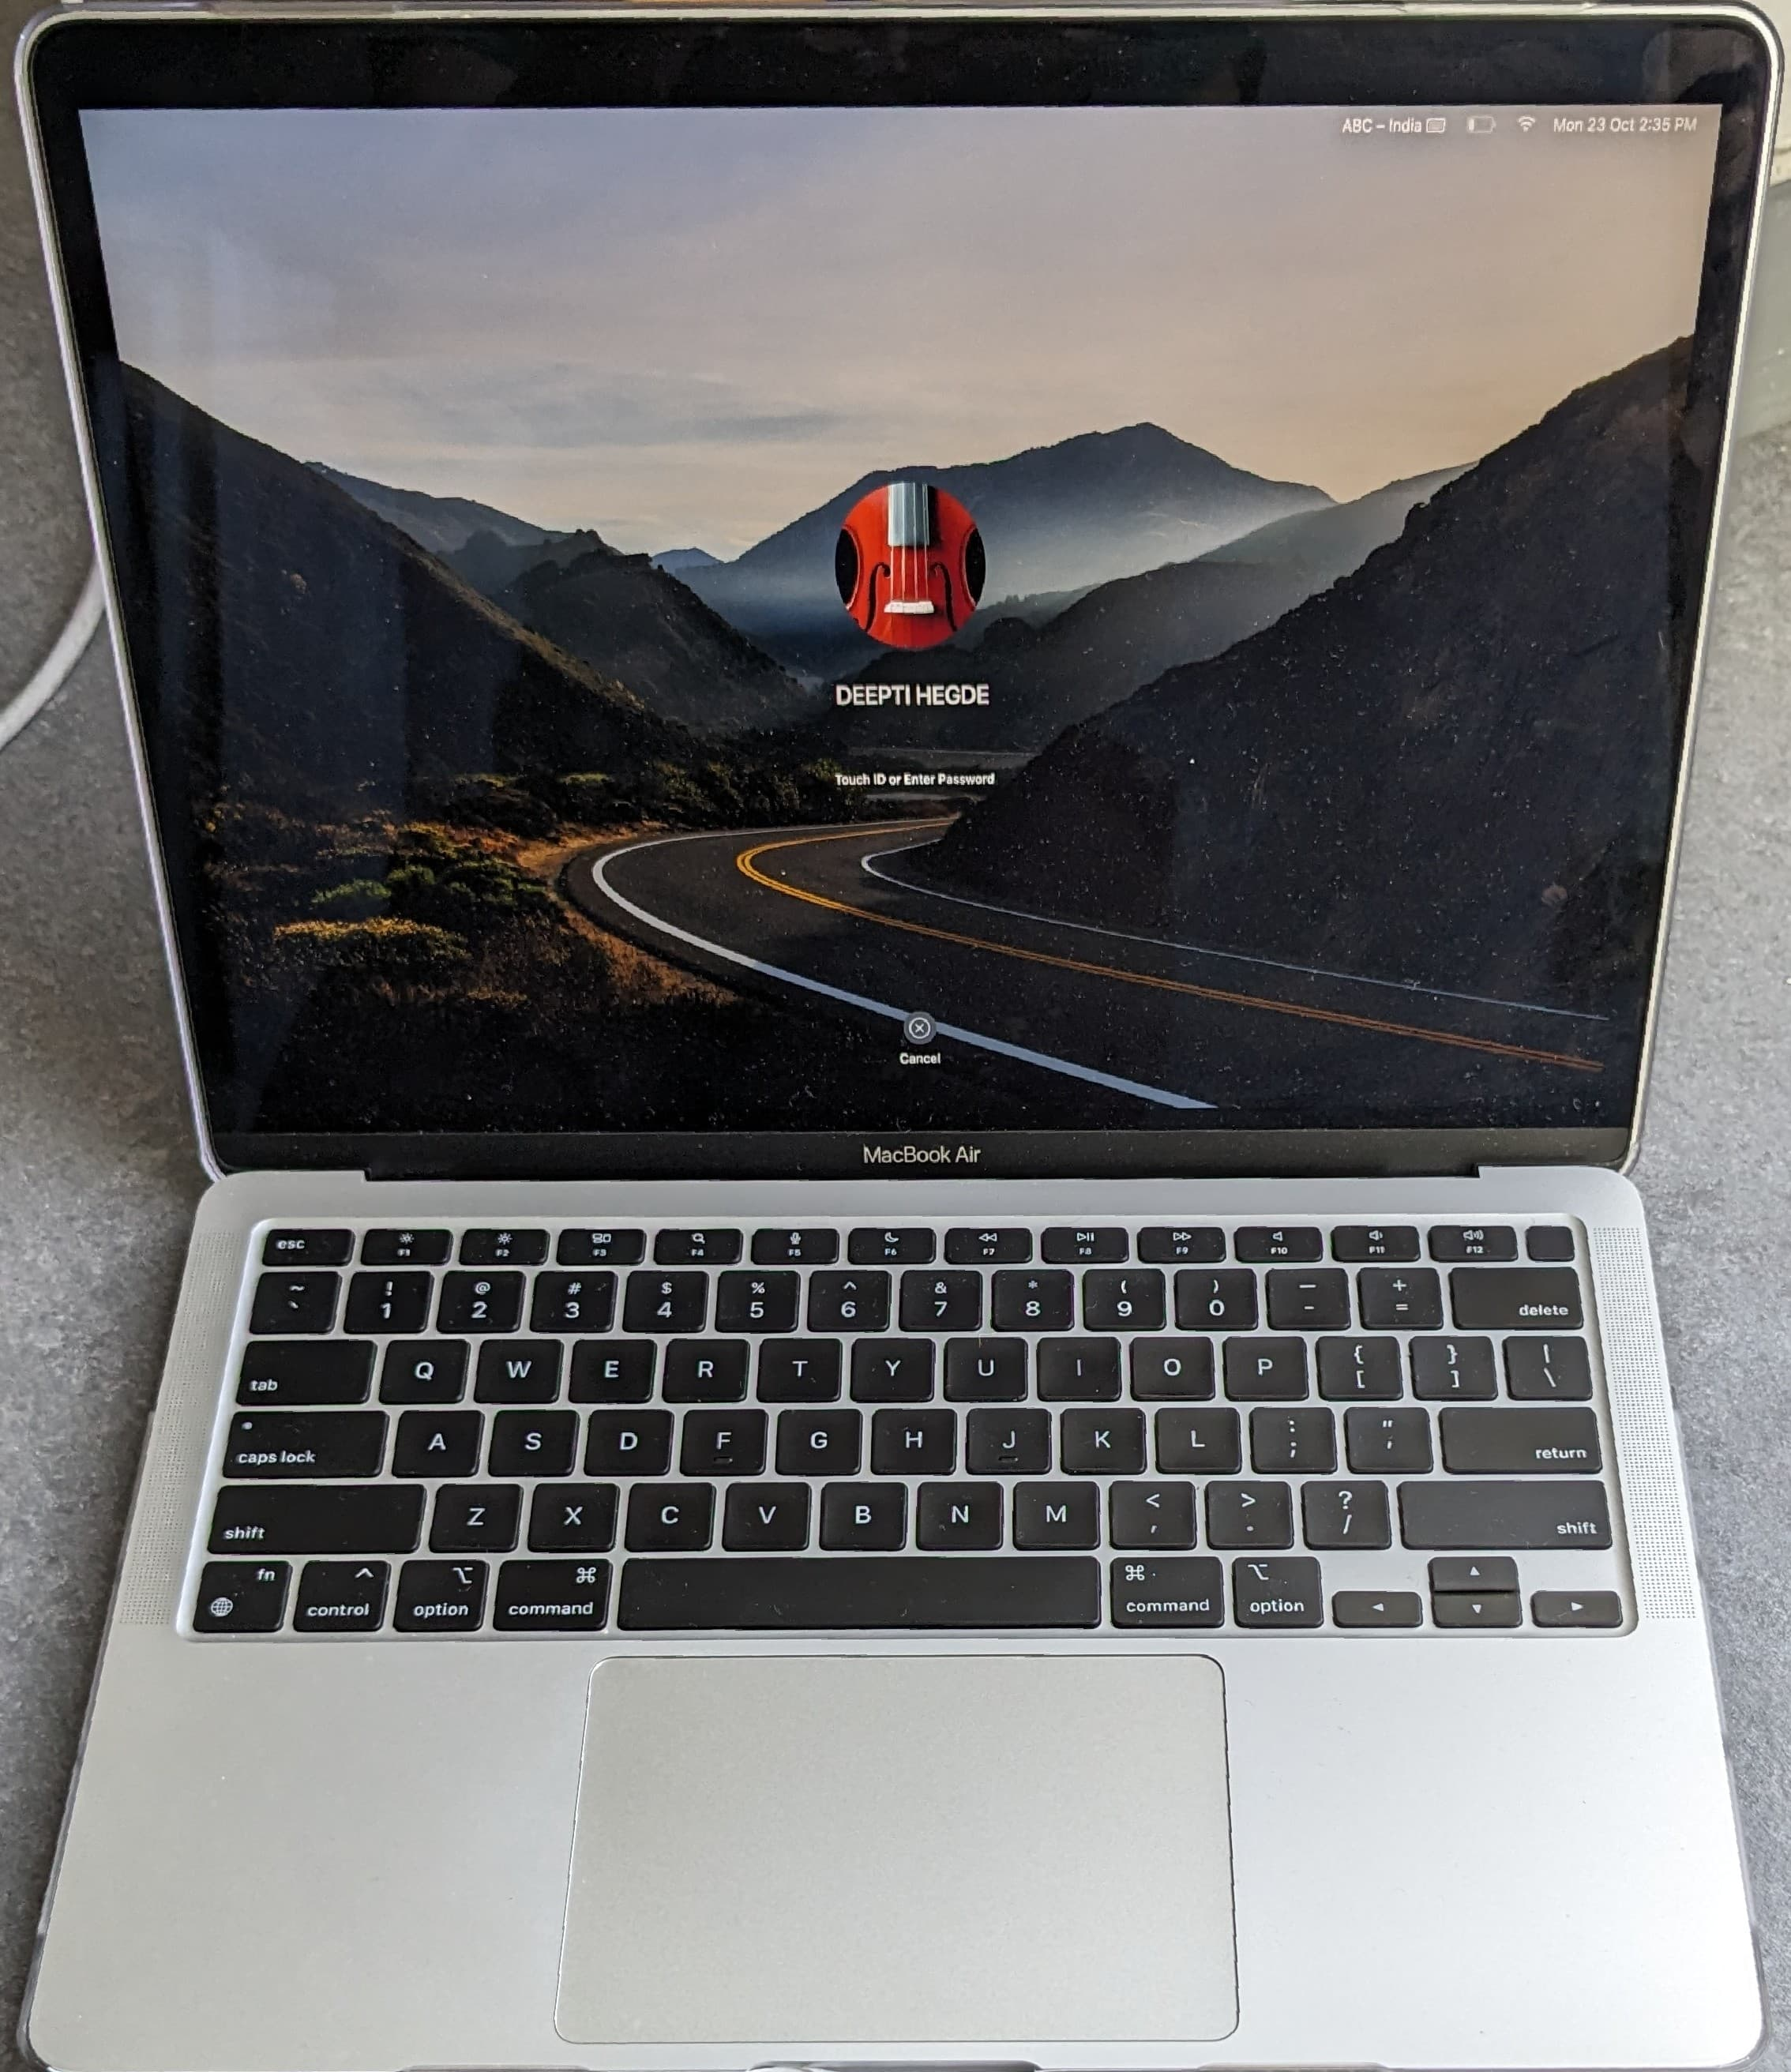
\includegraphics[width=0.2\textwidth]{Images/BillofMaterials/Laptop} & Laptop for software and final output & 1 \\
		
		\hline
		
		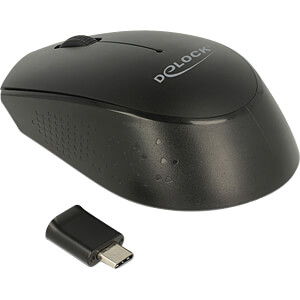
\includegraphics[width=0.2\textwidth]{Images/BillofMaterials/Mouse} & Wireless bluetooth mouse & 1 \\
		
		\hline
		
	\end{tabular}
	
	\caption {Supplements}
	\label{Table 5.3}
\end{table}

The supplementary hardware table \ref{Table 5.3} enhances the project by incorporating devices that support user interaction and software management.  

The laptop serves as the central hub for software development and the primary output display. It plays a pivotal role in programming the Arduino Nano, debugging, and real-time performance monitoring. Additionally, a wireless Bluetooth mouse complements the laptop by providing precise control and navigation, ensuring a seamless and user-friendly experience during interactions with the system.


\FILE{requirements.txt}
